\documentclass[a4paper,14pt,oneside,openany]{article}


\usepackage{listings}
\usepackage{indentfirst} 

\usepackage{fontspec}     
\setmainfont{CMU Serif}   
\newfontfamily\cyrillicfonttt{DejaVu Sans Mono} 
\usepackage{polyglossia}
\setdefaultlanguage{russian}
\setotherlanguage{english}

\renewcommand{\lstlistingname}{Листинг}
% Отображение страницы
\usepackage{geometry} % размеры листа и отступов
\geometry{
	left=12mm,
	top=25mm,
	right=15mm,
	bottom=17mm,
	marginparsep=0mm,
	marginparwidth=0mm,
	headheight=10mm,
	headsep=7mm,
	nofoot}
\usepackage{afterpage,fancyhdr} % настройка колонтитулов
\pagestyle{fancy}
\fancypagestyle{style}{ % создание нового стиля style
	\fancyhf{} % очистка колонтитулов
	\fancyhead[LO, RE]{} % название документа наверху
	\fancyhead[RO, LE]{\leftmark} % название section наверху
	\fancyfoot[RO, LE]{\thepage} % номер страницы справа внизу на нечетных и слева внизу на четных
	\renewcommand{\headrulewidth}{0.25pt} % толщина линии сверху
	\renewcommand{\footrulewidth}{0pt} % толцина линии снизу
}
\fancypagestyle{plain}{ % создание нового стиля plain -- полностью пустого
	\fancyhf{}
	\renewcommand{\headrulewidth}{0pt}
}
\fancypagestyle{title}{ % создание нового стиля title -- для титульной страницы
	\fancyhf{}
	\fancyhead[C]{{\footnotesize
			Министерство образования и науки Российской Федерации\\
			Федеральное государственное автономное образовательное учреждение высшего образования
	}}
	\fancyfoot[C]{{\large 
			Санкт-Петербург, \the\year
	}}
	\renewcommand{\headrulewidth}{0pt}
}

% Математика
\usepackage{amsmath, amsfonts, amssymb, amsthm} % Набор пакетов для математических текстов
%\usepackage{dmvnbase} % мехматовский пакет latex-сокращений
\usepackage{cancel} % зачеркивание для сокращений
% Рисунки и фигуры
\usepackage{graphicx}        
% \usepackage[unicode]{hyperref} % Was: \usepackage[unicode,pdftex]{hyperref}
\usepackage{wrapfig, subcaption} % вставка фигур, обтекая текст
\usepackage{caption} % для настройки подписей
\captionsetup{figurewithin=none,labelsep=period, font={small,it}} % настройка подписей к рисункам
% Рисование
\usepackage{tikz} % рисование
\usepackage{circuitikz}
\usepackage{pgfplots} % графики
% Таблицы
\usepackage{multirow} % объединение строк
\usepackage{multicol} % объединение столбцов
% Остальное
\usepackage{enumitem} % нормальное оформление списков
\usepackage{awesomebox}
\usepackage{tabularx}
\usepackage{hyperref} % гиперссылки
\usepackage{cleveref} % гиперссылки2

% Настройки стиля для листинга
\lstdefinestyle{mystyle}{
backgroundcolor=\color{gray!10!white},
basicstyle=\ttfamily,
language=Python,
numbers=left,
numberstyle=\small,
numbersep=5pt,
breaklines=true,
showstringspaces=false,
keywordstyle=\color{blue},
commentstyle=\color{green!40!black},
stringstyle=\color{green!40!black},
frame=single,
rulecolor=\color{black},
tabsize=2,
basicstyle=\small\ttfamily,
}


\setlist{itemsep=0.15cm,topsep=0.15cm,parsep=1pt} % настройки списков
% Теоремы, леммы, определения...
\theoremstyle{definition}
\newtheorem{Def}{Определение}
\newtheorem*{Axiom}{Аксиома}
\theoremstyle{plain}
\newtheorem{Th}{Теорема}
\newtheorem{Lem}{Лемма}
\newtheorem{Cor}{Следствие}
\newtheorem{Ex}{Пример}
\theoremstyle{remark}
\newtheorem*{Note}{Замечание}
\newtheorem*{Solution}{Решение}
\newtheorem*{Proof}{Доказательство}

\DeclareMathOperator{\sinc}{sinc}
\DeclareMathOperator{\Si}{Si}

% Свои команды
\newcommand{\comb}[1]{\left[\hspace{-4pt}\begin{array}{l}#1\end{array}\right.\hspace{-5pt} } % совокупность уравнений
% Титульный лист
\usepackage{csvsimple-l3}
\newcommand*{\titlePage}{
	\thispagestyle{title}
	\begingroup
	\begin{center}
		\begin{figure}[h]
			\centering
			
\includegraphics[width=0.2\linewidth]{./media/logo.jpg}
		\end{figure}
		
		Университет ИТМО
		
		\vspace*{15ex}


		{\Large \bfseries 
			Отчет по лабораторной работе
		}
\vspace*{2ex}
		
		{\Large \bfseries 
			по теме <<Формы представления линейных динамических систем>>
		}
\vspace*{2ex}
		
		{\Large
			по дисциплине Линейные системы автоматического управления
		}

\vspace*{2ex}
		{\Large
			Вариант 8
		}

	\end{center}
	\vspace*{18ex}
	\begin{flushright}
		{\large 
			Выполнил:\\
			Поляков А. А.\\                        
		}
		
		\vspace*{5ex}
		
		{\large 
			Преподаватель:\\
			Пашенко Артем Витальевич
		}
	\end{flushright}	
	\newpage
	\setcounter{page}{2}
	\endgroup
}

\begin{document}
\titlePage
\pagestyle{style}
\newpage

\tableofcontents* 


\section{Задание 1. Одноканальная система в форме вход-выход}
 
\subsection{Условие задания}

Рассмотреть математическую модель в форме дифференциального уравнения при коэффициентах 
$a_2 = 9, a_1 = 26, a_0 = 24, b_2 = 2, b_1 = 6$, $b _0 = 8$:

\begin{gather}
	\notag
	\dddot{y} + a_2\ddot{y} + a_1\dot{y} + a_0y = b_2\ddot{u} + b_1\dot{u} + b_0u\\
	\label{eq:dy_init}
	\dddot{y} + 9\ddot{y} + 26\dot{y} + 24y = 2\ddot{u} + 6\dot{u} + 8u
\end{gather}

На основании полученного дифференциального уравнения \eqref{eq:dy_init} с использованием блоков элементарных 
операций построить структурную схему одноканальной линейной динамической системы.

Выполнить моделирование при входном воздействии $u(t) = 1$ и нулевых начальных условиях 
$\ddot{y}(0)$, $\dot{y}(0)$, $y(0)$.

\subsection{Решение задания}

Рассмотрим математическую модель, дифференциальное уравнение 3-го порядка:

\begin{equation}
	\notag
	\dddot{y} + 9\ddot{y} + 26\dot{y} + 24y = 2\ddot{u} + 6\dot{u} + 8u
\end{equation}

\subsubsection{Преобразование математической модели}

На основании полученного дифференциального уравнения построим структурную схему одноканальной 
линейной динамической системы в среде \texttt{Simulink}. Сперва для удобства запишем дифференциальное 
уравнение в операторной форме. 

В качестве операторов будем использовать $p[f] = \frac{df}{dt}$ и $\frac{1}{p}[f] = \int_{0}^{\infty} f(t)dt$. 

Получим:

\begin{gather}
	\notag
	\dddot{y} + 9\ddot{y} + 26\dot{y} + 24y = 2\ddot{u} + 6\dot{u} + 8u,\\
	\notag
	p^3[y] + 9p^2[y] + 26p[y] + 24y = 2p^2[u] + 6p[u] + 8u\ \big| : p^3,\\
	\notag
	y + 9\frac{1}{p}[y] + 26\frac{1}{p^2}[y] + 24\frac{1}{p^3}[y] = 2\frac{1}{p}[u] + 6\frac{1}{p^2}[u] + 8\frac{1}{p^3}[u]\\
	\label{eq:dy_tran}
	y = - 9\frac{1}{p}[y] - 26\frac{1}{p^2}[y] - 24\frac{1}{p^3}[y] + 2\frac{1}{p}[u] + 6\frac{1}{p^2}[u] + 8\frac{1}{p^3}[u]
\end{gather}

Продолжим преобразовывать полученное выражение \eqref{eq:dy_tran}:

\begin{gather}
	\notag
	y = \frac{1}{p}\big[-9y - 26\frac{1}{p}[y] - 24\frac{1}{p^2}[y] + 2u + 6\frac{1}{p}[u] + 8\frac{1}{p^2}[u] \big]\\
	\notag
	y = \frac{1}{p}\big[-9y + 2u + \frac{1}{p}[ -26y + 6u - 24\frac{1}{p}[y] + 8\frac{1}{p}[u]] \big]\\
	\label{eq:dy_end}
	y = \frac{1}{p} \bigg[-9y + 2u + \frac{1}{p} \big[ -26y + 6u + \frac{1}{p}[-24y + 8u] \big] \bigg]
\end{gather}

\subsubsection{Построение структурной схемы и ее симуляция}

В итоге получаем преобразованное дифференциальное уравнение в операторной форме \eqref{eq:dy_end}. Попробуем составить 
структурную схему, используя элементарные операции, в \texttt{Simulink}. Получим схему: 

% \begin{figure}[!ht]
% 	\centering
% 	\includegraphics[width=1\linewidth]{./media/tsk1/simul.jpg}
% 	\caption{Структурная схема в \texttt{Simulink}}
% 	\label{fig:simul}
% \end{figure}

% Далее посмотрим на сигналы функций $u(t)$ \eqref{fig:graph_u(t)} и $y(t)$ \eqref{fig:graph_y(t)}, получаемые после симуляции схемы \eqref{fig:simul}. 

% Отметим, что сигнал $u(t)$ равен 1. Сигнал $y(t)$ можно охарактиризовать быстрым ростом, после чего принимает какое-то \textit{установленное} 
% значение.

% \notebox{
% 	В процессе выполнения был испробован вариант построения схемы с использованием передаточной функции. Результаты полностью совпадают, можно ознакомиться 
% 	на изображениях \eqref{fig:simul_per} и \eqref{fig:graph_y(t)_per}.
% }

% \begin{figure}[!ht]
% 	\centering
% 	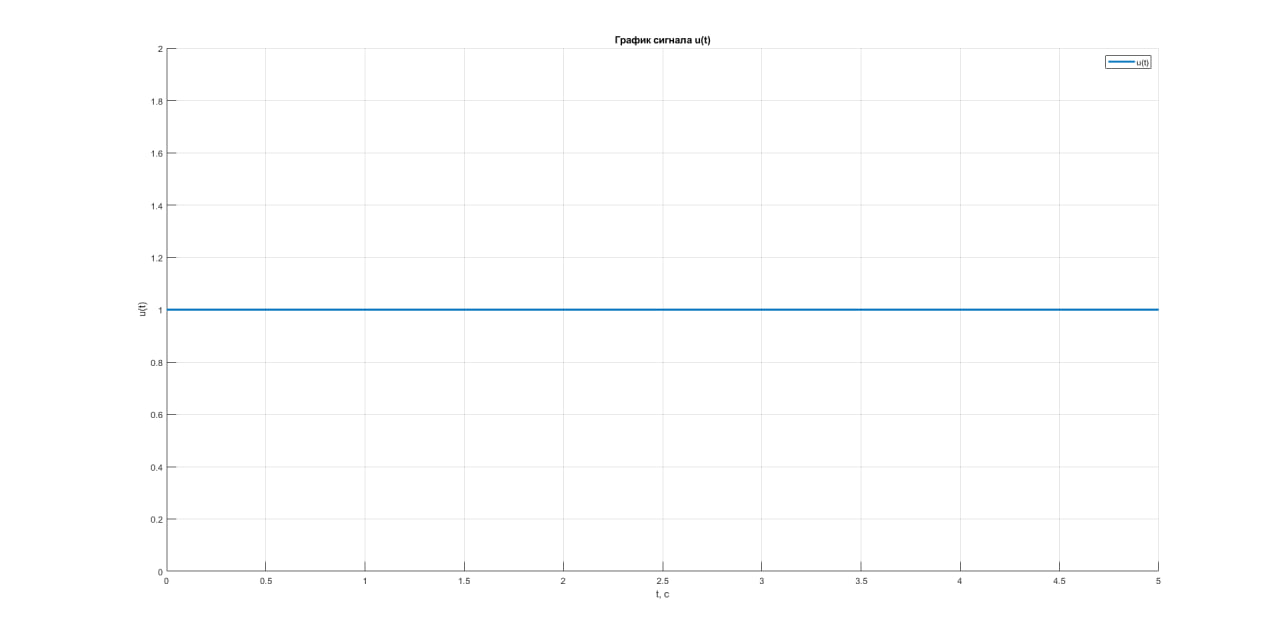
\includegraphics[width=1\linewidth]{./media/tsk1/graph_u(t).jpg}
% 	\caption{Сигнал $u(t)$}
% 	\label{fig:graph_u(t)}
% \end{figure}

% \begin{figure}[!ht]
% 	\centering
% 	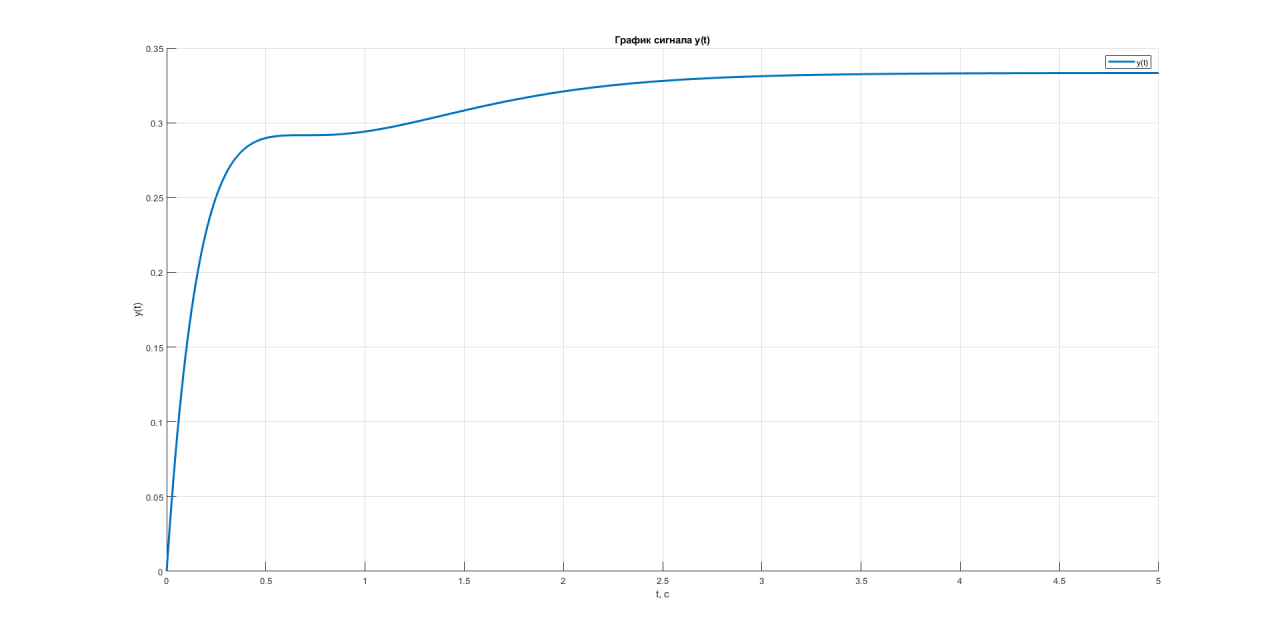
\includegraphics[width=1\linewidth]{./media/tsk1/graph_y(t).jpg}
% 	\caption{Сигнал $y(t)$}
% 	\label{fig:graph_y(t)}
% \end{figure}

% \newpage

% \section{Задание 2. Переход от формы В-В к форме В-С-В}

% \subsection{Условие задания}

% Для системы \eqref{eq:dy_init} определить передаточную функцию $W(p)$ и построить математические модели В-С-В в:

% \begin{enumerate}
% 	\item 
% 	Канонической управляемой форме
% 	\item
% 	Канонической наблюдаемой форме 
% 	\item
% 	Канонической диагональной форме 
% \end{enumerate}

% Для каждой из полученных моделей В-С-В построить структурные схемы с использованием блоков элементраных операций. 

% Выполнить моделирование четырех полученных форм представления системы при входном воздействии $u(t) = 1$ и нулевых начальных 
% условиях. 

% \subsection{Решение задания}

% Определим передаточную функцию системы \eqref{eq:dy_init}, затем определим разные формы этой системы.

% \subsubsection{Получение передаточной функции}

% Для нахождения передаточной функции запишем уравнение системы \eqref{eq:dy_init} в операторной форме, после чего получим:

% \begin{gather}
% 	\notag
% 	\dddot{y} + 9\ddot{y} + 26\dot{y} + 24y = 2\ddot{u} + 6\dot{u} + 8u,\\
% 	\notag
% 	p^3[y] + 9p^2[y] + 26p[y] + 24y = 2p^2[u] + 6p[u] + 8u\ \big| : p^3,\\
% 	\label{eq:w_p}
% 	W(p) = \frac{2p^2 + 6p + 8}{p^3 + 9p^2 + 26p + 24}
% \end{gather}

% Заметим, что формально при переходе к передаточной функции мы должны были прибавить общее решение левой части уравнения, но 
% из-за того, что нулевые условия системы равные нулю, это решение будет равняться 0.

% Благодаря передаточной функции $W(p)$ можно определить динамический порядок системы $max(m, n) = max(2, 3) = 3$, относительный 
% динамический порядок $n - m = 3 - 2 = 1$ и проверить условие физической реализуемости $n \geq{} m, 3 \geq{} m \to{}$ система физически 
% реализуема.

% \subsubsection{Построение канонической управляемой формы}

% Для того, чтобы представить дифференциальное уравнения в канонической управляемой форме необходимо совершить следующий переход:

% \begin{equation*}
% 	\dddot{y} + a_2\ddot{y} + a_1\dot{y} + a_0y = b_2\ddot{u} + b_1\dot{u} + b_0u\\
% \end{equation*}

% \begin{equation*}
% 	\begin{bmatrix}
% 		\dot{x_1}\\
% 		\dot{x_2}\\
% 		\dot{x_3}\\
% 	\end{bmatrix}
% 	=
% 	\begin{bmatrix}
% 		0 & 1 & 0\\
% 		0 & 0 & 1\\
% 		-a_0 & -a_1 & -a_2\\
% 	\end{bmatrix}
% 	\begin{bmatrix}
% 		x_1\\
% 		x_2\\
% 		x_3\\
% 	\end{bmatrix}
% 	+
% 	\begin{bmatrix}
% 		0\\
% 		0\\
% 		1\\
% 	\end{bmatrix}
% 	u
% \end{equation*}

% \begin{equation*}
% 	y = 
% 	\begin{bmatrix}
% 		b_0 & b_1 & b_2\\
% 	\end{bmatrix}
% 	\begin{bmatrix}
% 		x_1\\
% 		x_2\\
% 		x_3\\
% 	\end{bmatrix}
% \end{equation*}

% С учетом нашей системы \eqref{eq:dy_init} получим системы в канонической управляемой форме:

% \begin{equation}
% 	\label{eq:kan_upr}
% 	\begin{bmatrix}
% 		\dot{x_1}\\
% 		\dot{x_2}\\
% 		\dot{x_3}\\
% 	\end{bmatrix}
% 	=
% 	\begin{bmatrix}
% 		0 & 1 & 0\\
% 		0 & 0 & 1\\
% 		-24 & -26 & -9\\
% 	\end{bmatrix}
% 	\begin{bmatrix}
% 		x_1\\
% 		x_2\\
% 		x_3\\
% 	\end{bmatrix}
% 	+
% 	\begin{bmatrix}
% 		0\\
% 		0\\
% 		1\\
% 	\end{bmatrix}
% 	u
% \end{equation}

% \begin{equation*}
% 	y = 
% 	\begin{bmatrix}
% 		8 & 6 & 2\\
% 	\end{bmatrix}
% 	\begin{bmatrix}
% 		x_1\\
% 		x_2\\
% 		x_3\\
% 	\end{bmatrix}
% \end{equation*}

% \subsubsection{Структурная схема канонической управляемой формы}

% В среде Matlab Simulink построим структурную схему: 

% \begin{figure}[!ht]
% 	\centering
% 	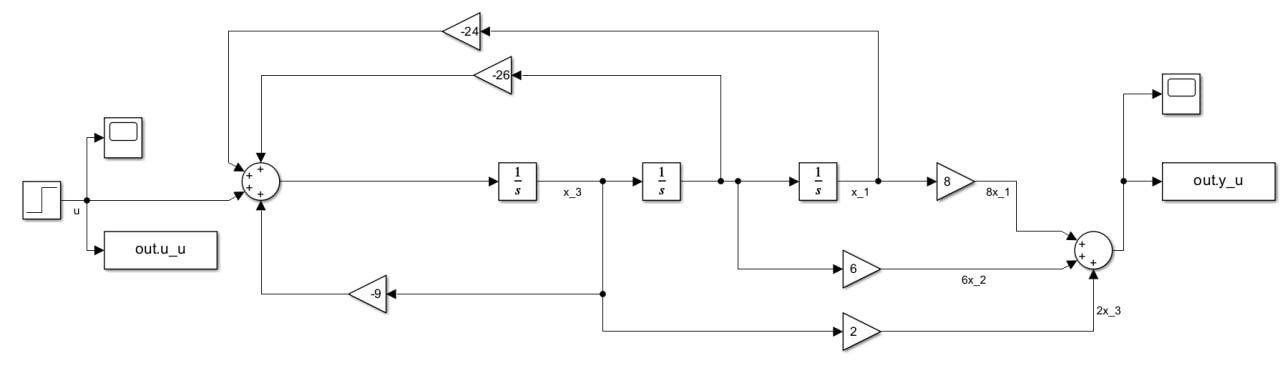
\includegraphics[width=1\linewidth]{./media/tsk2/simul_upr.jpg}
% 	\caption{Структурная схема в управляемой форме}
% 	\label{fig:simul_upr}
% \end{figure}

% \subsubsection{Моделирование схемы канонической управляемой формы}

% Построим график $y(t)$ и сравним его с тем, что получился в системе В-В \eqref{fig:graph_y(t)}:

% \begin{figure}[!ht]
% 	\centering
% 	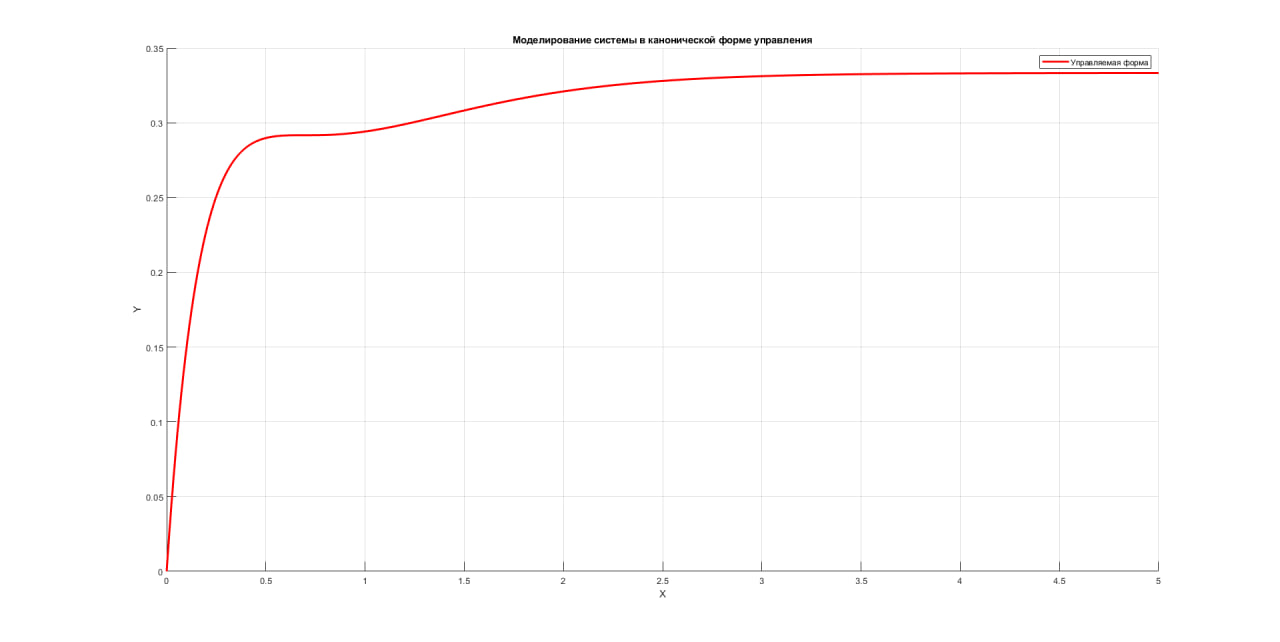
\includegraphics[width=1\linewidth]{./media/tsk2/y_t_ypr.jpg}
% 	\caption{Сигнал $y(t)$ по схеме канонической управляемой формы}
% 	\label{fig:graph_y_t_upr}
% \end{figure}

% График действительно имеет такой же вид, что и в системе В-В. 

% \subsubsection{Построение канонической наблюдаемой формы}

% Для того, чтобы представить дифференциальное уравнения в канонической наблюдаемоей форме необходимо совершить следующий переход 
% (он похож на предыдущий переход, но он \textit{как бы перевернутый}):

% \begin{equation*}
% 	\dddot{y} + a_2\ddot{y} + a_1\dot{y} + a_0y = b_2\ddot{u} + b_1\dot{u} + b_0u\\
% \end{equation*}

% \begin{equation*}
% 	\begin{bmatrix}
% 		\dot{x_1}\\
% 		\dot{x_2}\\
% 		\dot{x_3}\\
% 	\end{bmatrix}
% 	=
% 	\begin{bmatrix}
% 		0 & 0 & -a_0\\
% 		1 & 0 & -a_1\\
% 		0 & 1 & -a_2\\
% 	\end{bmatrix}
% 	\begin{bmatrix}
% 		x_1\\
% 		x_2\\
% 		x_3\\
% 	\end{bmatrix}
% 	+
% 	\begin{bmatrix}
% 		b_0\\
% 		b_1\\
% 		b_2\\
% 	\end{bmatrix}
% 	u
% \end{equation*}

% \begin{equation*}
% 	y = 
% 	\begin{bmatrix}
% 		0 & 0 & 1\\
% 	\end{bmatrix}
% 	\begin{bmatrix}
% 		x_1\\
% 		x_2\\
% 		x_3\\
% 	\end{bmatrix}
% \end{equation*}

% С учетом нашей системы \eqref{eq:dy_init} получим системы в канонической наблюдаемой форме:

% \begin{equation}
% 	\label{eq:kan_nab}
% 	\begin{bmatrix}
% 		\dot{x_1}\\
% 		\dot{x_2}\\
% 		\dot{x_3}\\
% 	\end{bmatrix}
% 	=
% 	\begin{bmatrix}
% 		0 & 0 & -24\\
% 		1 & 0 & -26\\
% 		0 & 1 & -9\\
% 	\end{bmatrix}
% 	\begin{bmatrix}
% 		x_1\\
% 		x_2\\
% 		x_3\\
% 	\end{bmatrix}
% 	+
% 	\begin{bmatrix}
% 		8\\
% 		6\\
% 		2\\
% 	\end{bmatrix}
% 	u
% \end{equation}

% \begin{equation*}
% 	y = 
% 	\begin{bmatrix}
% 		0 & 0 & 1\\
% 	\end{bmatrix}
% 	\begin{bmatrix}
% 		x_1\\
% 		x_2\\
% 		x_3\\
% 	\end{bmatrix}
% \end{equation*}

% \subsubsection{Структурная схема канонической наблюдаемой формы}

% В среде Matlab Simulink построим структурную схему: 

% \begin{figure}[!ht]
% 	\centering
% 	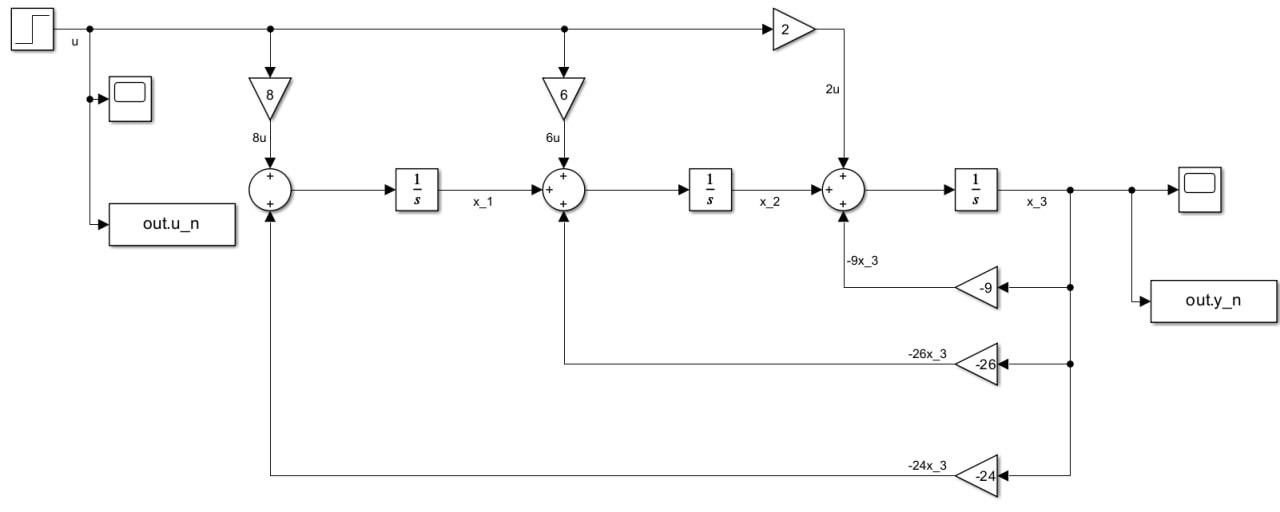
\includegraphics[width=1\linewidth]{./media/tsk2/simul_nabl.jpg}
% 	\caption{Структурная схема в наблюдаемой форме}
% 	\label{fig:simul_nabl}
% \end{figure}

% \newpage

% \subsubsection{Моделирование схемы канонической наблюдаемой формы}

% Построим график $y(t)$ и сравним его с тем, что получился в системе В-В \eqref{fig:graph_y(t)}:

% \begin{figure}[!ht]
% 	\centering
% 	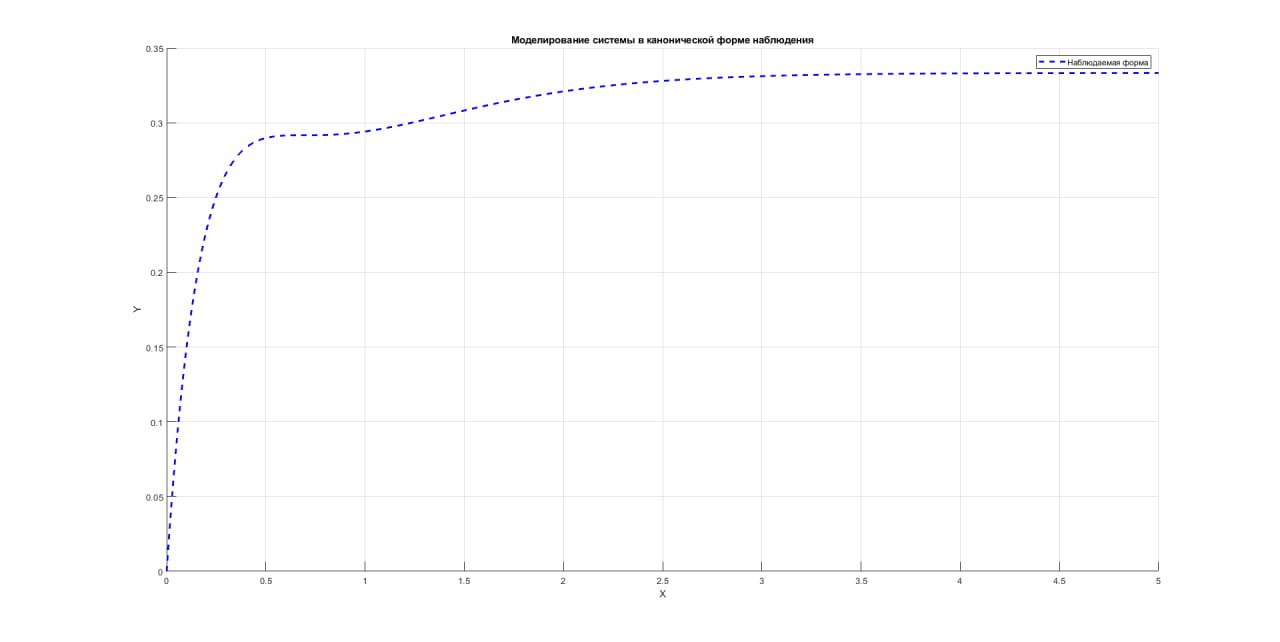
\includegraphics[width=1\linewidth]{./media/tsk2/y_t_nab.jpg}
% 	\caption{Сигнал $y(t)$ по схеме канонической наблюдаемой формы}
% 	\label{fig:graph_y_t_nabl}
% \end{figure}

% График аналогично схож с ожидаемым.

% \subsubsection{Построение канонической диагональной формы}

% Для построения канонической диагональной формы нам необходимо взять передаточную функцию \eqref{eq:w_p} и 
% разложить ее на простейшие дроби. Затем записать результат в виде матриц:

% \begin{equation*}
% 	W(p) = \frac{b_2p^2 + b_1p + b_0}{p^3 + a_2p^2 + a_1p + a_0} = \frac{\beta_1\gamma_1}{p - \lambda_1} + \frac{\beta_2\gamma_2}{p - \lambda_2} + \frac{\beta_3\gamma_3}{p - \lambda_3}
% \end{equation*}

% \begin{equation*}
% 	\begin{bmatrix}
% 		\dot{x_1}\\
% 		\dot{x_2}\\
% 		\dot{x_3}\\
% 	\end{bmatrix}
% 	=
% 	\begin{bmatrix}
% 		\lambda_1 & 0 & 0\\
% 		0 & \lambda_2 & 0\\
% 		0 & 0 & \lambda_3\\
% 	\end{bmatrix}
% 	\begin{bmatrix}
% 		x_1\\
% 		x_2\\
% 		x_3\\
% 	\end{bmatrix}
% 	+
% 	\begin{bmatrix}
% 		\beta_0\\
% 		\beta_1\\
% 		\beta_2\\
% 	\end{bmatrix}
% 	u
% \end{equation*}

% \begin{equation*}
% 	y = 
% 	\begin{bmatrix}
% 		\gamma_1 & \gamma_2 & \gamma_3\\
% 	\end{bmatrix}
% 	\begin{bmatrix}
% 		x_1\\
% 		x_2\\
% 		x_3\\
% 	\end{bmatrix}
% \end{equation*}

% Перейдем к нашему случаю и разложим полученную ранее передаточную функцию \eqref{eq:w_p} на простейшие дроби:

% \begin{equation*}
% 	W(p) = \frac{2p^2 + 6p + 8}{p^3 + 9p^2 + 26p + 24} = \frac{2}{p + 2} + \frac{-8}{p + 3} + \frac{8}{p + 4}
% \end{equation*}

% Отсюда получим каноническую диагональную форму:

% \begin{equation*}
% 	\begin{bmatrix}
% 		\dot{x_1}\\
% 		\dot{x_2}\\
% 		\dot{x_3}\\
% 	\end{bmatrix}
% 	=
% 	\begin{bmatrix}
% 		-2 & 0 & 0\\
% 		0 & -3 & 0\\
% 		0 & 0 & -4\\
% 	\end{bmatrix}
% 	\begin{bmatrix}
% 		x_1\\
% 		x_2\\
% 		x_3\\
% 	\end{bmatrix}
% 	+
% 	\begin{bmatrix}
% 		1\\
% 		-4\\
% 		4\\
% 	\end{bmatrix}
% 	u
% \end{equation*}

% \begin{equation*}
% 	y = 
% 	\begin{bmatrix}
% 		2 & 2 & 2\\
% 	\end{bmatrix}
% 	\begin{bmatrix}
% 		x_1\\
% 		x_2\\
% 		x_3\\
% 	\end{bmatrix}
% \end{equation*}

% \subsubsection{Структурная схема канонической диагональной формы}

% В среде Matlab Simulink построим структурную схему: 

% \begin{figure}[!ht]
% 	\centering
% 	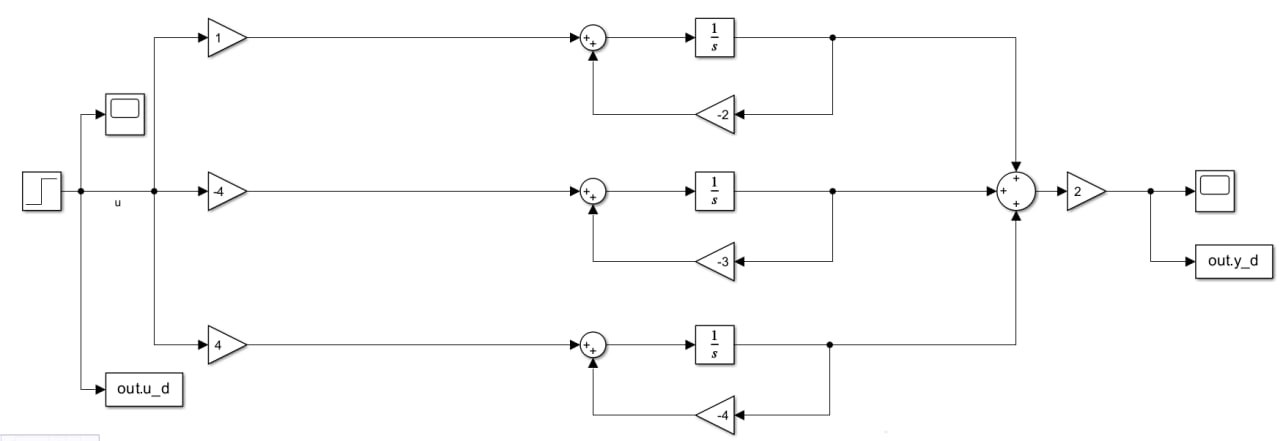
\includegraphics[width=1\linewidth]{./media/tsk2/simul_diag.jpg}
% 	\caption{Структурная схема в диагональной форме}
% 	\label{fig:simul_diag}
% \end{figure}

% \newpage

% \subsubsection{Моделирование схемы канонической диагональной формы}

% Построим график $y(t)$ и сравним его с тем, что получился в системе В-В \eqref{fig:graph_y(t)}:

% \begin{figure}[!ht]
% 	\centering
% 	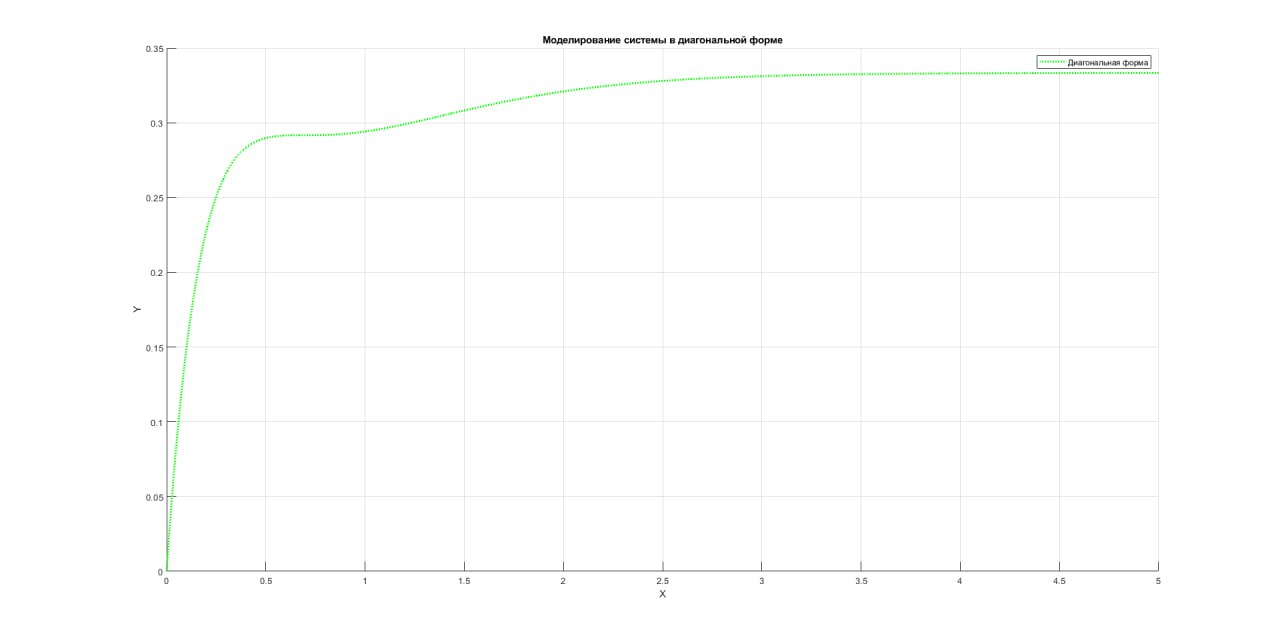
\includegraphics[width=1\linewidth]{./media/tsk2/y_t_diag.jpg}
% 	\caption{Сигнал $y(t)$ по схеме диагональной формы}
% 	\label{fig:graph_y_t_diag}
% \end{figure}

% График аналогично схож с ожидаемым.

% \subsubsection{Сравнение графиков различных форм}

% Теперь сравним все полученные результаты моделирования \eqref{fig:all_graphs}. Ожидаемые результат -- все графики должны быть идентичными, 
% так как при переходе от формы В-В к форме В-С-В мы меняем только вид схемы, меняем \textit{точку зрения} на систему.

% \newpage

% \begin{figure}[!ht]
% 	\centering
% 	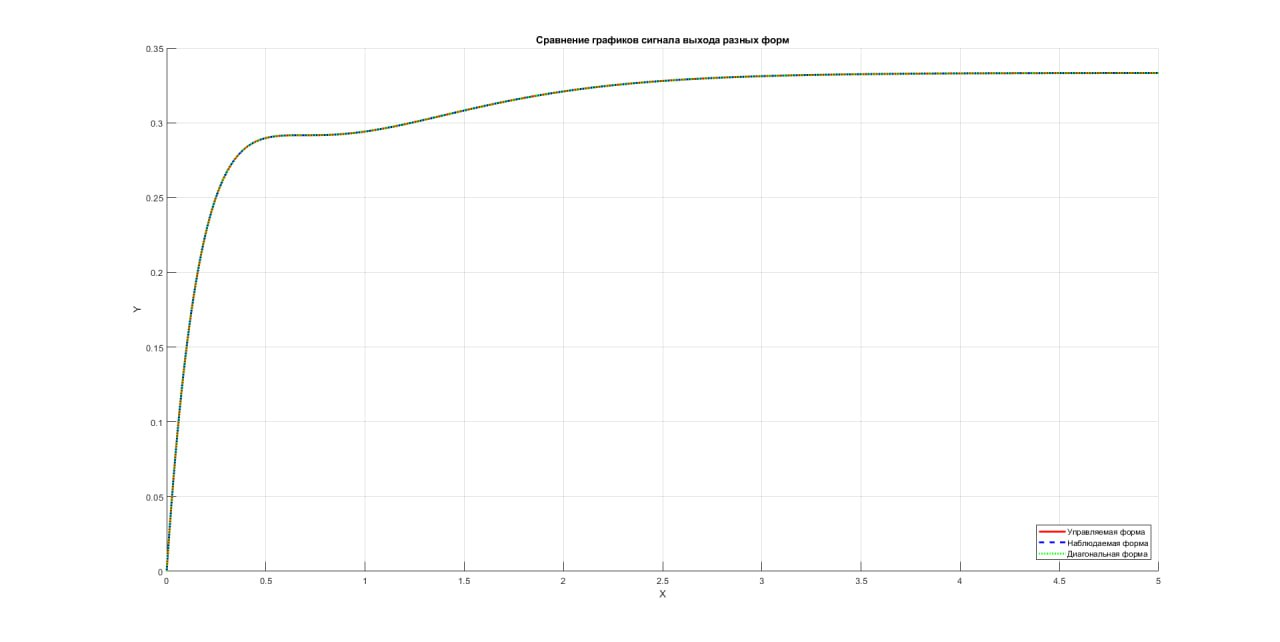
\includegraphics[width=1\linewidth]{./media/tsk2/all_graph.jpg}
% 	\caption{Сравнение выходных сигналов $y(t)$}
% 	\label{fig:all_graphs}
% \end{figure}

%  И посмотрим на входные сигналы $u(t)$ разных форм системы:

% \begin{figure}[!ht]
% 	\centering
% 	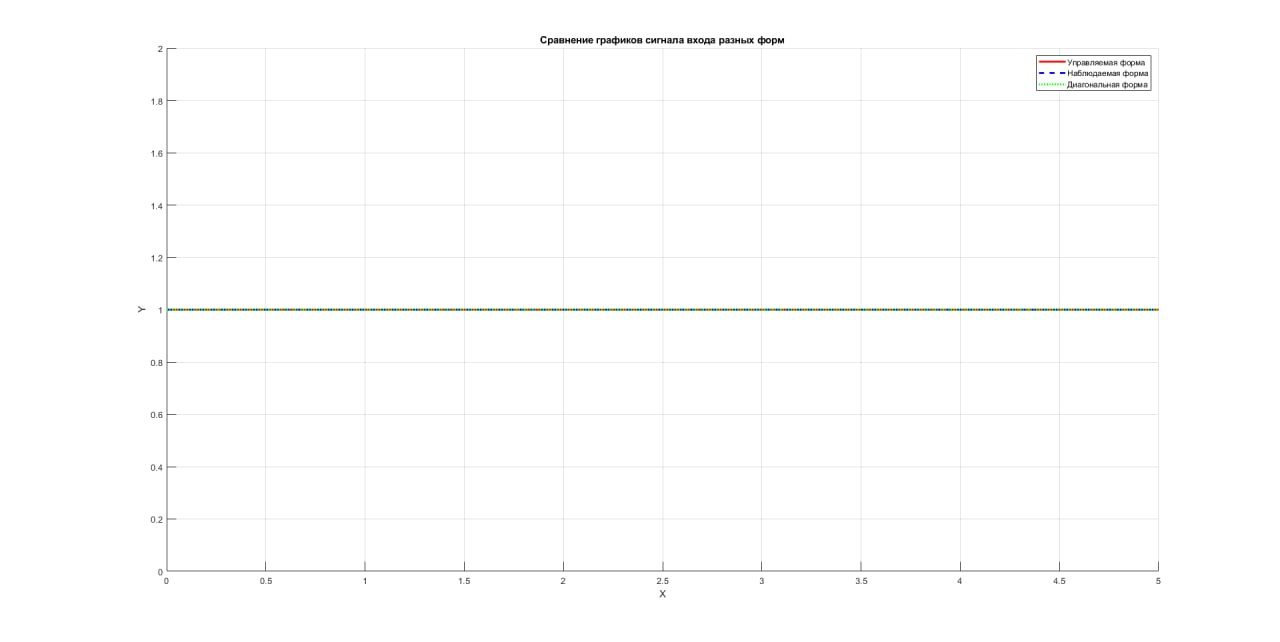
\includegraphics[width=1\linewidth]{./media/tsk2/all_graph_u.jpg}
% 	\caption{Сравнение выходных сигналов $u(t)$}
% 	\label{fig:all_graphs_u}
% \end{figure}

% Ожидаемо графики $y(t)$ и $u(t)$ полностью совпадают, что подтверждает теорию.

% \section{Задание 3. Многоканальная система в форме вход-выход}

% \subsection{Условие задания}

% Взять коэффициенты $a_{11}(p) = p + 17, a_{12}(p) = p + 5, a_{21}(p) = p + 4$, 
% $a_{21}(p) = p + 2, b_{11}(p) = 6, b_{12}(p) = 8, b_{21}(p) = 4, b_{21}(p) = 3$ и рассмотреть систему 

% \begin{equation*}
% 	A(p)y(t) = B(p)u(t),
% \end{equation*}

% где 

% \begin{equation*}
% 	A(p) = 
% 	\begin{bmatrix}
% 		a_{11}(p) & a_{12}(p)\\
% 		a_{21}(p) & a_{22}(p)\\
% 	\end{bmatrix},
% 	B(p) = 
% 	\begin{bmatrix}
% 		b_{11}(p) & b_{12}(p)\\
% 		b_{21}(p) & b_{22}(p)\\
% 	\end{bmatrix},
% \end{equation*}

% Определить для данной системы передаточную матрицу $W(p)$ и построить структурную схему 
% двухканальной линейной динамической системы (при построении структурной схемы в данном задании 
% приемлемо отводить каждой передаточной функции отдельный блок, не дробя на блоки элементарных 
% операций).

% Выполнить моделирование при входных воздействиях $u_1(t) = 1$ и $u_2(t) = 2\sin(t)$ и нулевых 
% начальных условиях. 

% \subsection{Решение задания}

% При выданных коэффициентах система будет иметь вид:

% \begin{equation}
% 	\label{eq:scheme}
% 	A(p)y(t) = B(p)u(t),
% \end{equation}

% \begin{equation*}
% 	A(p) = 
% 	\begin{bmatrix}
% 		p + 17 & p + 5\\
% 		p + 4 & p + 2\\
% 	\end{bmatrix},
% 	B(p) = 
% 	\begin{bmatrix}
% 		6 & 8\\
% 		4 & 3\\
% 	\end{bmatrix},
% \end{equation*}

% \subsubsection{Получение передаточной функции}

% Из схемы \eqref{eq:scheme} выразим передаточную систему:

% \begin{gather*}
% 	A(p)y(t) = B(p)u(t)\\
% 	y(t) = A^{-1}(p)B(p)u(t)
% \end{gather*}

% Откуда получаем, что

% \begin{gather*}\\
% 	W(p) = A^{-1}(p)B(p)
% 	y(t) = W(p)u(t)
% \end{gather*}

% Найдем обратную матрицу к матрице $A(p)$:

% \begin{equation*}
% 	A^{-1}(p) = \frac{(A^*)^T}{detA}
% \end{equation*}

% Сперва найдем определитель матрицы $A$:

% \begin{equation*}
% 	detA = (p + 17)(p + 2) - (p + 5)(p + 4)
% \end{equation*}

% Найдем транспонированную матрицу алгебраических дополнения $A^*$:

% \begin{equation*}
% 	A^* = 
% 	\begin{bmatrix}
% 		p + 2 & -p - 5\\
% 		-p - 4 & p + 17\\
% 	\end{bmatrix}
% \end{equation*}

% Тогда обратная матрица имеет вид: 

% \begin{equation*}
% 	A^{-1} = 
% 	\begin{bmatrix}
% 		\frac{p + 2}{10p + 14} & \frac{-p - 5}{10p + 14}\\
% 		\frac{-p - 4}{10p + 14} & \frac{p + 17}{10p + 14}\\
% 	\end{bmatrix}
% \end{equation*}

% Тогда передаточная матрица $W(p)$ имеет вид:

% \begin{equation}
% 	W(p) = A^{-1}(p)B(p) = 
% 	\begin{bmatrix}
% 		\frac{p + 2}{10p + 14} & \frac{-p - 5}{10p + 14}\\
% 		\frac{-p - 4}{10p + 14} & \frac{p + 17}{10p + 14}\\
% 	\end{bmatrix} 
% 	\begin{bmatrix}
% 		6 & 8\\
% 		4 & 3\\
% 	\end{bmatrix}
% 	=
% 	\begin{bmatrix}
% 		\frac{p - 4}{5p + 7} & \frac{5p + 1}{10p + 14}\\
% 		\frac{-p + 22}{5p + 7} & \frac{-5p + 19}{10p + 14}\\
% 	\end{bmatrix}
% \end{equation}

% Теперь построим схемы каждой отдельной передаточной функции $W_{11}$, $W_{12}$, $W_{21}$, $W_{22}$.

% \subsubsection{Построение схемы передаточной функции $W_{11}$}

% Для начала преобразуем передаточную функцию:

% \begin{equation*}
% 	W_{11} = \frac{p - 4}{5p + 7}
% \end{equation*}

% \begin{gather*}
% 	5p[y] + 7y = p[u] - 4u\\
% 	5p[y] = p[u] - 4u - 7y\\
% 	y = \frac{1}{5}u - \frac{4}{5}\frac{1}{p}[u] - \frac{7}{5}\frac{1}{p}[y]\\
% 	y = \frac{1}{5}u + \frac{1}{p}[-\frac{4}{5}u - \frac{7}{5}y]
% \end{gather*}

% Структурная схема имеет вид:

% \begin{figure}[!ht]
% 	\centering
% 	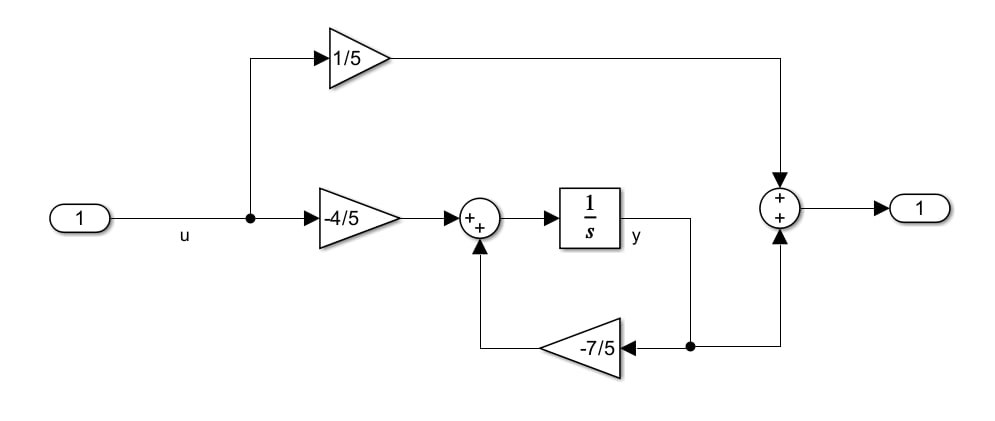
\includegraphics[width=1\linewidth]{./media/tsk3/w11.jpg}
% 	\caption{Структурная схема передаточной функции $W_{11}$}
% \end{figure}

% \subsubsection{Построение схемы передаточной функции $W_{12}$}

% Для начала преобразуем передаточную функцию:

% \begin{equation*}
% 	W_{12} = \frac{5p + 1}{10p + 14}
% \end{equation*}

% \begin{gather*}
% 	10p[y] + 14y = 5[u] + u\\
% 	10p[y] = 5p[u] + u - 14y\\
% 	y = \frac{5}{10}u + \frac{1}{10}\frac{1}{p}[u] - \frac{14}{10}\frac{1}{p}[y]\\
% 	y = \frac{5}{10}u + \frac{1}{p}[\frac{1}{10}u - \frac{14}{10}y]
% \end{gather*}

% Структурная схема имеет вид:

% \begin{figure}[!ht]
% 	\centering
% 	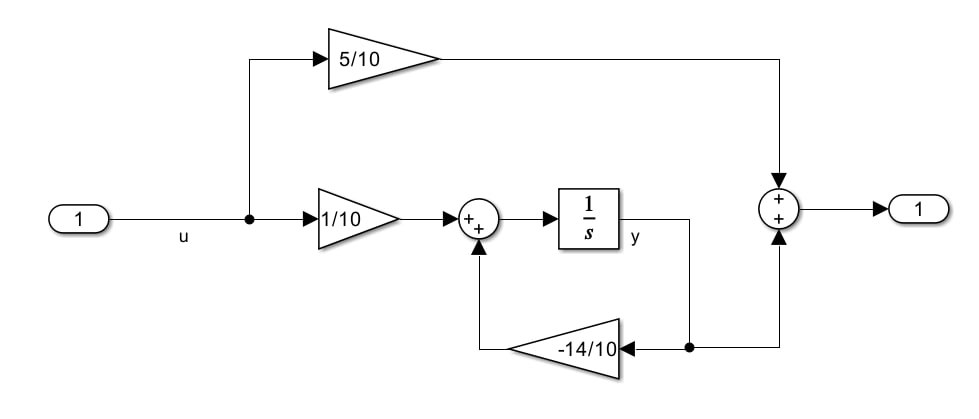
\includegraphics[width=1\linewidth]{./media/tsk3/w12.jpg}
% 	\caption{Структурная схема передаточной функции $W_{12}$}
% \end{figure}

% \subsubsection{Построение схемы передаточной функции $W_{21}$}

% Для начала преобразуем передаточную функцию:

% \begin{equation*}
% 	W_{21} = \frac{-p + 22}{5p + 7}
% \end{equation*}

% \begin{gather*}
% 	5p[y] + 7y = -p[u] + 22u\\
% 	5p[y] = -p[u] + 22u - 7y\\
% 	y = -\frac{1}{5}u + \frac{22}{5}\frac{1}{p}[u] - \frac{7}{5}\frac{1}{p}[y]\\
% 	y = -\frac{1}{5}u + \frac{1}{p}[\frac{22}{5}u - \frac{7}{5}y]
% \end{gather*}

% \newpage

% Структурная схема имеет вид:

% \begin{figure}[!ht]
% 	\centering
% 	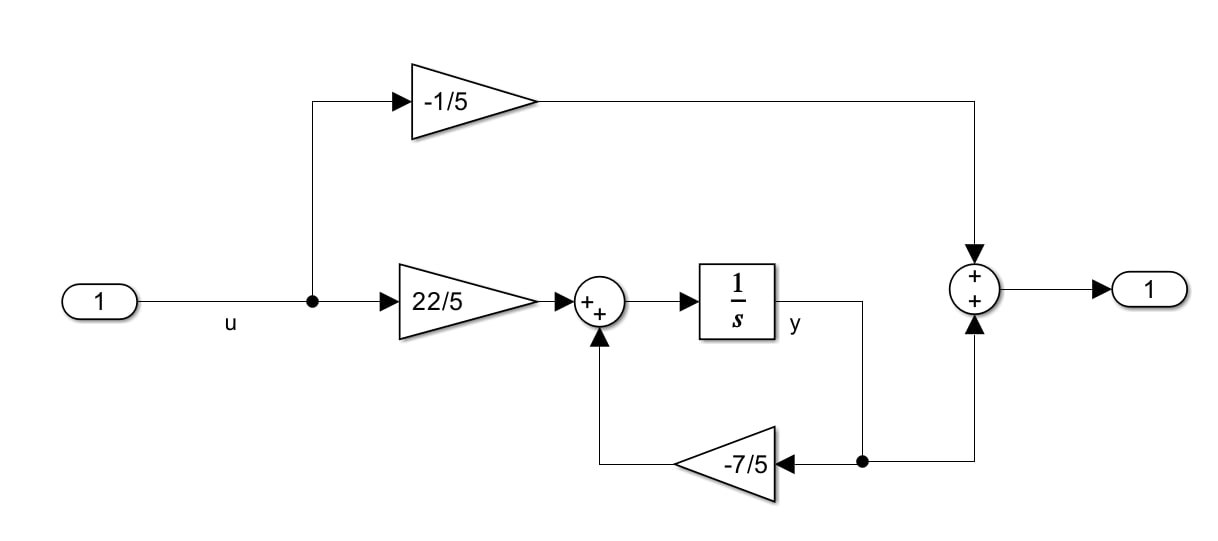
\includegraphics[width=1\linewidth]{./media/tsk3/w21.jpg}
% 	\caption{Структурная схема передаточной функции $W_{21}$}
% \end{figure}

% \subsubsection{Построение схемы передаточной функции $W_{22}$}

% Для начала преобразуем передаточную функцию:

% \begin{equation*}
% 	W_{22} = \frac{-5p + 19}{10p + 14}
% \end{equation*}

% \begin{gather*}
% 	10p[y] + 14y = -5p[u] + 19u\\
% 	5p[y] = -5p[u] + 19u - 14y\\
% 	y = -u + \frac{19}{5}\frac{1}{p}[u] - \frac{14}{5}\frac{1}{p}[y]\\
% 	y = -u + \frac{1}{p}[\frac{19}{5}u - \frac{14}{5}y]
% \end{gather*}

% \newpage

% Структурная схема имеет вид:

% \begin{figure}[!ht]
% 	\centering
% 	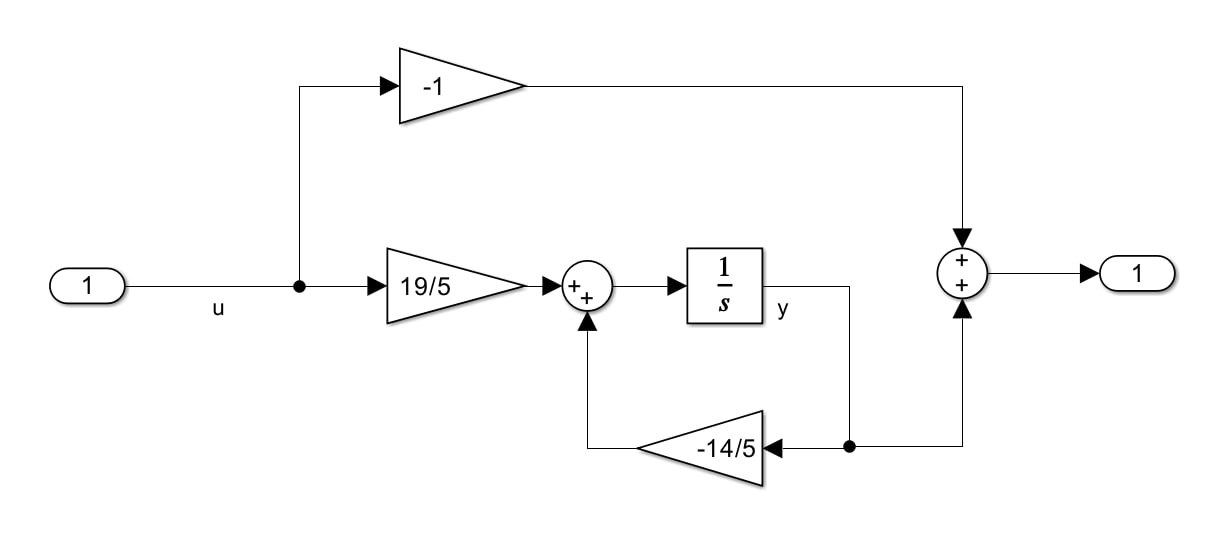
\includegraphics[width=1\linewidth]{./media/tsk3/w22.jpg}
% 	\caption{Структурная схема передаточной функции $W_{22}$}
% \end{figure}

% \subsubsection{Анализ результатов}

% На вход подавалось два воздействия $u_1(t)$ и $u_2(t)$:

% \begin{figure}[!ht]
% 	\centering
% 	\includegraphics[width=1\linewidth]{./media/tsk3/u(t).jpg}
% 	\caption{Входные сигналы $u(t)$}
% \end{figure}

% \newpage

% На выходе имеет два сигнала $y_1(t)$ и $y_2(t)$:

% \begin{figure}[!ht]
% 	\centering
% 	\includegraphics[width=1\linewidth]{./media/tsk3/y(t).jpg}
% 	\caption{Выходные сигналы $y(t)$}
% \end{figure}

% \section{Задание 4. Многоканальная система в форме вход-состояние-выход}

% \subsection{Условие задания}

% Рассмотреть систему: 

% \begin{equation*}
% 	\begin{cases}
% 		\dot{x} = Ax + Bu,\\
% 		y = Cx
% 	\end{cases},
% \end{equation*}

% где 

% \begin{equation*}
% 	A = 
% 	\begin{bmatrix}
% 		0 & -2\\
% 		1 & -7\\
% 	\end{bmatrix}
% 	\ \ \ \ 
% 	B = 
% 	\begin{bmatrix}
% 		3 & 0\\
% 		2 & 7\\
% 	\end{bmatrix}
% 	\ \ \ \ 
% 	C = 
% 	\begin{bmatrix}
% 		0 & 7\\
% 		4 & 6\\
% 	\end{bmatrix}
% \end{equation*}

% Построить для данной системы структурную схему с использованием блоков элементарных операций. На структурной 
% схеме должны быть явно обозначены каналы, соответствующие компонентам вектора состояния $x$.

% Выполнить моделирование при входных воздействиях $u_1(t) = 1$ и $u_2(t) = 2\sin(t)$ и нулевом начальном 
% значении вектора состояния.

% \subsection{Решение задания}


% Система дана в матричном виде, преобразуем его к виду уравнения, для удобства создания структурной 
% схемы:

% \begin{equation*}
% 	\begin{bmatrix}
% 		\dot{x_1}\\
% 		\dot{x_2}\\ 
% 	\end{bmatrix}
% 	=
% 	\begin{bmatrix}
% 		0 & -2\\
% 		1 & -7\\
% 	\end{bmatrix}
% 	\begin{bmatrix}
% 		x_1\\
% 		x_2
% 	\end{bmatrix}
% 	+
% 	\begin{bmatrix}
% 		3 & 0\\
% 		2 & 7\\
% 	\end{bmatrix}
% 	\begin{bmatrix}
% 		u_1\\
% 		u_2
% 	\end{bmatrix}, \ \ \ \
% 	\begin{bmatrix}
% 		y_1\\
% 		y_2\\
% 	\end{bmatrix}
% 	=
% 	\begin{bmatrix}
% 		0 & 7\\
% 		4 & 6\\
% 	\end{bmatrix}
% 	\begin{bmatrix}
% 		x_1\\
% 		x_2
% 	\end{bmatrix}
% \end{equation*}

% \begin{gather*}
% 	\dot{x_1} = -2x_2 + 3u_1\ \ \ \ \dot{x_2} = x_1 - 7x_2 + 2u_1 + 7u_2\\ 
% 	y_1 = 7x_2 \ \ \ \ y_2 = 4x_1 + 6x_2\\
% \end{gather*}

% Структурная схема будет иметь вид:

% \begin{figure}[!ht]
% 	\centering
% 	\includegraphics[width=1\linewidth]{./media/tsk4/simul.jpg}
% 	\caption{Структурная схема системы}
% \end{figure}

% \newpage

% Сигнал для выхода будет иметь вид:

% \begin{figure}[!ht]
% 	\centering
% 	\includegraphics[width=1\linewidth]{./media/tsk4/y(t).jpg}
% 	\caption{Сигналы входов $y_1(t)$ и $y_2(t)$}
% \end{figure}

% Сигналы входов будет иметь вид:

% \begin{figure}[!ht]
% 	\centering
% 	\includegraphics[width=1\linewidth]{./media/tsk4/u(t).jpg}
% 	\caption{Сигналы входов $u_1(t)$ и $u_2(t)$}
% \end{figure}

% \newpage

% По сигналам входа нельзя однозначно сказать, что система является стабильной, поэтому увеличим время моделирования 
% и проверим результат:

% \begin{figure}[!ht]
% 	\centering
% 	\includegraphics[width=1\linewidth]{./media/tsk4/y(t)ispr.png}
% 	\caption{Сигналы входов $y_1(t)$ и $y_2(t)$}
% \end{figure}

% Сигналы входов будет иметь вид:

% \begin{figure}[!ht]
% 	\centering
% 	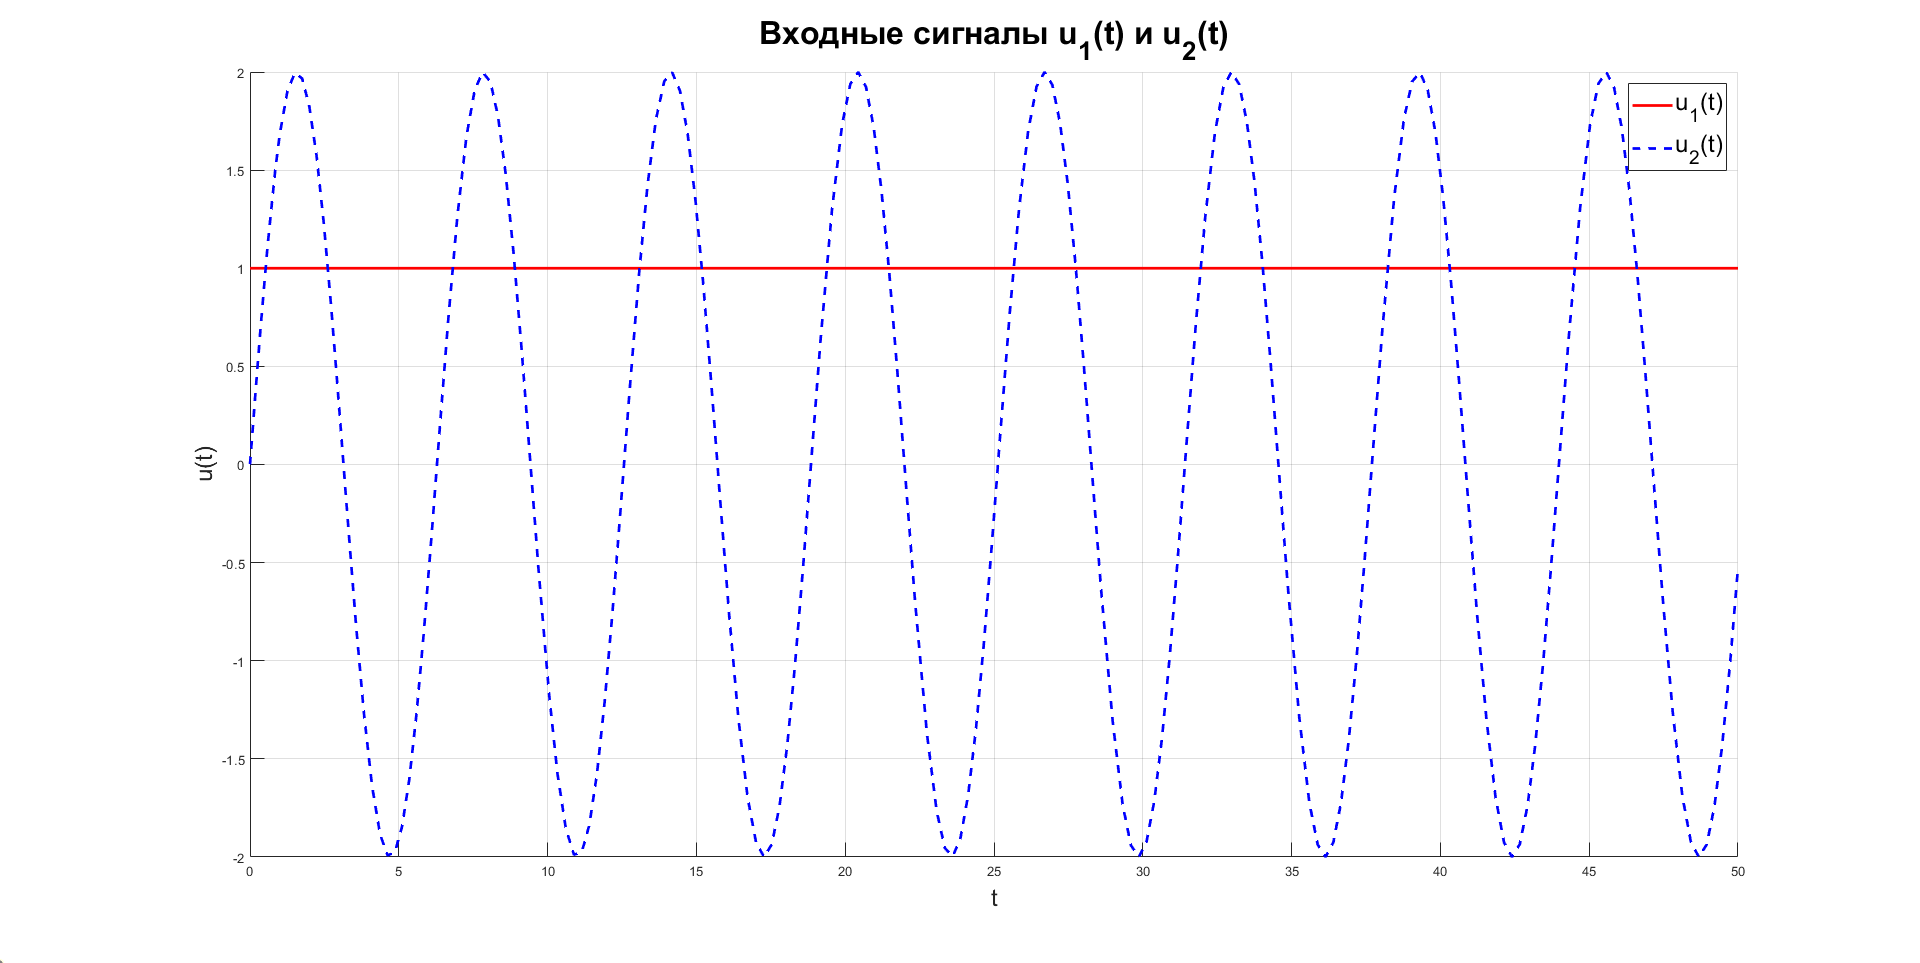
\includegraphics[width=1\linewidth]{./media/tsk4/u(t)ispr.png}
% 	\caption{Сигналы входов $u_1(t)$ и $u_2(t)$}
% \end{figure}

% Видно, что система спустя время становится стабильной.

% \newpage

% \section{Вывод}

% В процессе выполнения лабораторной работы были получены знания по работе со средой \texttt{Matlab Simulink}, 
% получен опыт в создании структурных схем некоторых линейных систем в различных входах В-В или В-С-В, используя 
% только лишь элементарные блоки: интегратор, усилитель и сумматор. 

% На практике было подтверждено теоретическое высказывание: форма В-В может быть представлена бесконечным 
% количеством различных форм В-С-В в одноканальном случае (существует бесконечное количество вариантов представить 
% схему В-В схемой В-С-В с аналогичным действием).


% \newpage
% \section{Приложение}

% \begin{figure}[!ht]
% 	\centering
% 	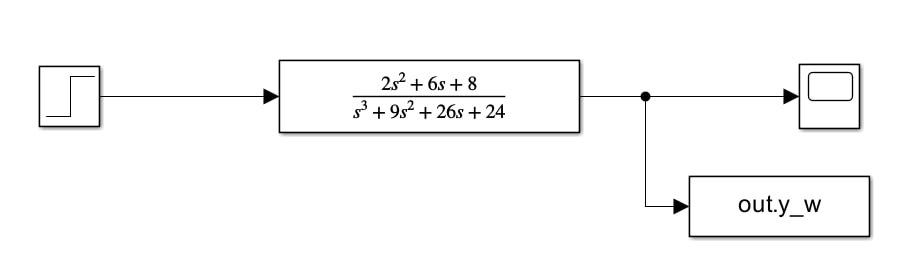
\includegraphics[width=1\linewidth]{./media/tsk1/simul_per.jpg}
% 	\caption{Схема с использованием передаточной функции}
% 	\label{fig:simul_per}
% \end{figure}

% \begin{figure}[!ht]
% 	\centering
% 	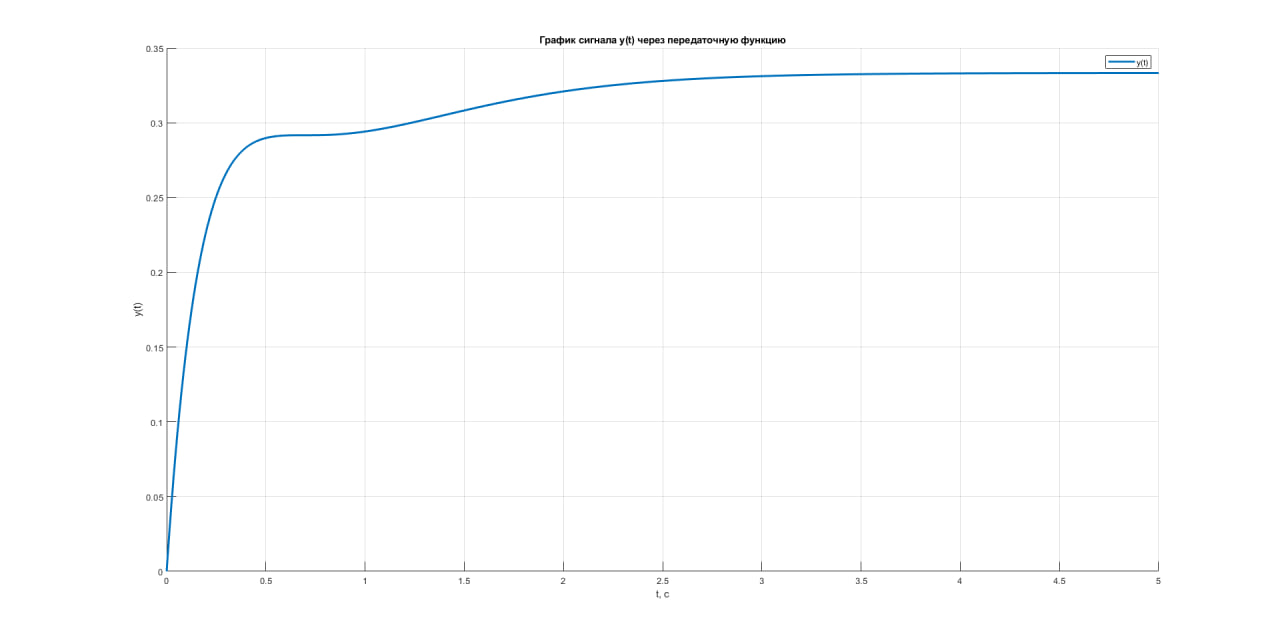
\includegraphics[width=1\linewidth]{./media/tsk1/graph_y(t)_per.jpg}
% 	\caption{Сигнал $y(t)$, полученный с передаточной функцией}
% 	\label{fig:graph_y(t)_per}
% \end{figure}



\end{document}
